\subsection{Introducción}
La implementación de la infraestructura de telecomunicaciones ha transformado numerosos aspectos de la vida cotidiana y el ámbito industrial, dando lugar a innovaciones que facilitan la comunicación y el control de diversos sistemas. Uno de estos avances es el Internet de las Cosas (IoT), que conecta objetos físicos a la red, permitiendo su monitoreo y control a través de dispositivos electrónicos y software. En este contexto, en el área de la apicultura se han adoptado tecnologías IoT para mejorar la gestión y el monitoreo de las colmenas, creando lo que se conoce como colmenas inteligentes.

En este capítulo se ofrece un marco teórico sobre los conceptos clave del internet, IoT y su aplicación en la apicultura. Se explora la arquitectura IoT, desglosada en sus siete capas fundamentales, y se examina la interacción de los sensores en estos sistemas. Además, se profundiza en el uso de IoT en las colmenas, destacando su capacidad para monitorear parámetros críticos como la temperatura, la humedad y el peso de la colmena, así como para detectar el enjambrado a través del análisis de sonidos específicos. También se proporciona una visión general sobre la inteligencia artificial y su potencial integración en sistemas IoT para optimizar el control y análisis de datos en la apicultura.
\subsection{Apicultura}
Se refiere a la crianza y explotación de abejas, de las cuales se obtienen productos como miel, cera y polen, y que al mismo tiempo realizan el servicio de polinización de plantas.

\subsection{Abejas}
Se refiere a un insecto social que durante su ciclo de vida se encarga de producir miel, cera y panal y polinizar plantas para apoyarlas en su reproducción, por lo cual se les considera de los insectos más importantes del planeta.  \cite{david_cramp}

\subsection{Colmena}
Una abeja no puede sobrevivir de manera individual, una abeja obrera no se puede reproducir y una abeja reina no puede construir o mantener una colmena ya que la estructura social de las abejas requiere de a las obreras, las reinas y los drones para sobrevivir, por lo cual se considera a la misma como un organismo independiente. \cite{david_cramp} En la figura~\ref{fig:abejas} se muestra una imagen ilustrativa de las 3 castas de abeja.

\begin{figure}[htbp]
  \centering
  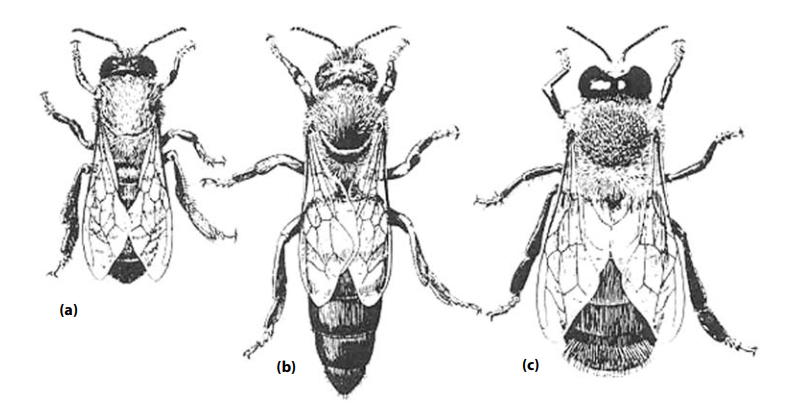
\includegraphics[width=0.75\textwidth]{assets/abejas.png}
  \caption{Castas de abejas. \cite{david_cramp}}
  \label{fig:abejas}
\end{figure}

Como se observa en la figura~\ref{fig:abejas}, las castas de abejas son las siguientes:
\begin{enumerate}
  \renewcommand\labelenumi{\alph{enumi})}
  \item \textbf{Obreras}: Estas se encargan de todas las tareas no relacionadas con la reproducción, incluyendo la construcción del panal, la recolección de polen, la producción de miel, entre otras actividades vitales para la colmena.
  \item \textbf{Reinas}: Son la única hembra completa de la colonia; su única responsabilidad es reproducirse y poner huevos.
  \item \textbf{Drones}: Similar a la reina; su única responsabilidad es reproducirse con reinas de otras colonias.
\end{enumerate}

\subsection{Temperatura de la colmena}
Una colmena debe de mantener una temperatura cercana a los 34 grados centígrados, para lograr esto pueden implementar ciertos mecanismos de regulación de temperatura. \cite{david_cramp}
Cuando las abejas necesitan elevar la temperatura, generan una capa de abejas vivas alrededor de la reina, después proceden a vibrar con el objetivo de producir calor. Para este proceso es necesario que la colmena cuente con suficiente alimento, además, se apoya del aislamiento de la colmena, ya sea natural o artificial, de modo natural, la miel y la cera son buenos aislantes. \cite{chadwick_alton_tennant_fitzmaurice_earl_2016}
Por otro lado, las abejas suelen iniciar un aleteo con sus alas para reducir la temperatura dentro de la colmena. \cite{chadwick_alton_tennant_fitzmaurice_earl_2016}

\subsection{Humedad de la colmena}
La humedad tiene un papel importante en la prevención de enfermedades dentro de la colmena, por esta razón es de importancia para las abejas controlar esta propiedad, el mecanismo que utilizan las abejas en estos casos es utilizar sus alas como ventiladores para expulsar la humedad de la colmena. \cite{chadwick_alton_tennant_fitzmaurice_earl_2016}

\subsection{Peso de la colmena}
El peso es el principal factor utilizado por los apicultores para medir la cantidad en los almacenes de miel, de manera tradicional, los apicultores intentan levantar la colmena, en caso de no ser capaces, consideran que la miel esta lista para ser extraída \cite{chadwick_alton_tennant_fitzmaurice_earl_2016}, de manera precisa, se considera una extracción cuando el almacén de miel pesa cerca a los 40kg.\cite{david_cramp}

\subsection{Enjambrado}
El evento de enjambre sucede cuando una colonia de abejas ha sobrepasado el límite físico de la colmena en la que habita, este proceso comienza con la reina engendrando nuevas reinas y drones, después de esto un enjambre de abejas y drones emigran a un nuevo posible lugar en el cual comienza una nueva colmena. \cite{chadwick_alton_tennant_fitzmaurice_earl_2016}

Uno de los principales indicadores del enjambrado es el sonido que emiten las abejas, durante este proceso comienzan a emitir un sonido de vibración, este sonido es conocido por los apicultores y es la principal fuente de información que se obtiene sobre este proceso \cite{david_cramp} \cite{chadwick_alton_tennant_fitzmaurice_earl_2016}.

\subsection{Internet e IoT}

\subsubsection{Internet}
En el contexto actual, internet se refiere a una red global con varios protocolos de conectividad que permite comunicar paquetes de datos de dispositivos, mediante un sistema de rúters, a la red. \cite{kamal_2017}

\subsubsection{Rúter, router o enrutador}
Se refiere a un dispositivo capaz de almacenar direcciones y enlaces mediante las cuales se encarga de mandar paquetes de datos.\cite{kamal_2017}

\subsubsection{Internet de las cosas (IoT)}
El termino de internet de las coas, o IOT por sus siglas en inglés (Internet of things), se refiere al concepto de entrelazar objetos físicos dentro de una red de internet, mediante componentes electrónicos y sistemas de software, con el objetivo de permitir la comunicación entre ellos y monitorear o controlar un sistema físico. \cite{kamal_2017}

\subsubsection{Arquitectura IoT}
Este concepto se refiere a la forma de estructurar u diseñar un sistema IOT y estos se dividen en capas y son 7 principales
\begin{enumerate}
  \renewcommand\labelenumi{\arabic{enumi}.}
  \item Componentes físicos: sensores y controladores.
  \item Dispositivos de conectividad.
  \item Computación perimetral (análisis de datos y procesamiento).
  \item Persistencia de datos.
  \item Abstracción de datos (acceso y manipulación).
  \item Aplicación (reportes, análisis y control).
  \item Colaboración y procesos (usuarios y procesos comerciales).
\end{enumerate}
Estas capas sirven para estructurar y definir la arquitectura del sistema IOT.\cite{kamal_2017}


\subsubsection{Sensores}
El sistema IOT interactúa con sensores, dispositivos físicos con el objetivo de adquirir datos mediante la capacidad de reaccionar a parámetros físicos como la humedad, temperatura, presión y luz y convertirla en energía eléctrica capaz de interactuar con el sistema. Durante esta interacción es posible configurar los dispositivos de manera que se ajusten a los requerimientos de la aplicación.\cite{kamal_2017}

\subsubsection{Colmenas inteligentes}
Los términos Colmenas IOT o colmenas inteligentes se refieren a la adición de un sistema IOT a una colmena apícola, esto con el objetivo de monitorear los parámetros de la colonia de abejas y hacer accesible la información de manera que pueda ser procesada para conocer el estado de la colmena. \cite{open_source_beehives_project_iaac}

\subsection{Inteligencia artificial}

\subsubsection{Sistema inteligente}
Se refiere a un concepto abstracto en el cual se define a un sistema que actúa y razona de manera humana o de manera lógica \cite{russell_norvig_2022}. Es uno de los posibles métodos para procesar datos de un sistema IOT \cite{open_source_beehives_project_iaac}.

\subsubsection{Minería de datos}
Se refiere al proceso de aplicar métodos computacionales a grandes cantidades de datos con el objetivo de revelar información nueva, no trivial y relevante \cite{fayyad1996kdd}. Esto incluye la aplicación de algoritmos específicos para la extracción de patrones, la limpieza de datos, el preprocesamiento y la extracción de características.


\subsubsection{Preprocesamiento de datos}
El preprocesamiento de datos es una etapa en la minería de datos que consiste en preparar y limpiar el conjunto de datos con el objetivo de mejorar su calidad para que sean adecuados para el análisis o modelado. Esto implica corregir valores inválidos, eliminar columnas irrelevantes, manejar valores faltantes, ajustar datos inconsistentes, entre otros \cite{statistical_modeling_in_machine_learning_2023}.

\subsubsection{Aprendizaje automático}
El aprendizaje automático, o aprendizaje maquina, es una rama de la inteligencia artificial que se centra en desarrollar algoritmos capaces de aprender automáticamente a partir de los datos y mejorar su desempeño con la experiencia, sin ser programados explícitamente. Formalmente, se dice que un programa aprende de una experiencia $E$ respecto a una clase de tareas $T$ y una medida de desempeño $P$, si su desempeño en las tareas de $T$, medida por $P$, mejora con la experiencia $E$. En otras palabras, el desempeño del algoritmo en una tarea mejora conforme gana experiencia al realizarla \cite{mitchell1997machine}.


\subsubsection{Extracción de características}
La extracción de características es una técnica de preprocesamiento de datos utilizada en el aprendizaje máquina para transformar un conjunto de datos complejos y con muchas características, en un espacio más manejable y representativo. Se utiliza cuando hay demasiadas características ya sea para un análisis efectivo o para la visualización de datos \cite{richer_coelho_2013}.

\subsubsection{Características de audio}

\begin{itemize}
  \item \textbf{Zero Crossing Rate (ZCR):} Número de veces que la señal cruza el eje cero por unidad de tiempo. Indica la frecuencia de cambios en la señal, útil para distinguir sonidos ruidosos y tonales \cite{muller2015fmp}.

  \item \textbf{RMS (Root Mean Square):} Raíz cuadrada del promedio cuadrático de las muestras; mide energía promedio de la señal, útil para comparar su intensidad relativa entre segmentos \cite{sound_quality_heyboer2010}.

  \item \textbf{Energía:} Suma de los cuadrados de las amplitudes de la señal, representa la potencia o intensidad del sonido \cite{rabiner2010fundamentals}.

  \item \textbf{Entropía de energía:} Mide la distribución y variabilidad de la energía dentro de una señal, calculada usando entropía de Shannon sobre segmentos de energía \cite{li2017audio}.

  \item \textbf{Centroide espectral:} Promedio ponderado de las frecuencias presentes en una señal, que refleja el "brillo" percibido del sonido \cite{peeters2004large}.

  \item \textbf{Dispersión espectral:} Desviación estándar de la distribución espectral alrededor del centroide, indica la extensión del contenido frecuencial \cite{peeters2004large}.

  \item \textbf{Entropía espectral:} Entropía de Shannon aplicada a la densidad espectral de potencia, mide la complejidad del espectro \cite{jiang2011spectral}.

  \item \textbf{Flujo espectral:} Cambio en el espectro de potencia entre frames consecutivos, usado para detectar transiciones y dinámica en la señal \cite{foote2000novelty}.

  \item \textbf{Rolloff espectral:} Frecuencia debajo de la cual se acumula un porcentaje dado (e.g., 85\%) de la energía espectral, útil para distinguir sonidos agudos de graves \cite{tzanetakis2002musical}.

  \item \textbf{MFCC (1 a 13):} Coeficientes cepstrales calculados sobre la escala de frecuencias Mel, que modelan el timbre y la estructura espectral, ampliamente usados en reconocimiento de voz y análisis musical \cite{davis1980tassp}.
\end{itemize}


